\section{Mathematical Framework (Discussion)}\label{sec:c9s2}
\kant[5-11]

This section builds on the material in \cref{sec:c9s1}, \cref{ch:10} and the prior work of \citet{main-32}; see also \citep{main-6,main-16}.

\begin{equation}\label{eq:c9s2-a}
  I = \int_{0}^{1}\!\!\int_{0}^{1} \frac{\sin(\pi x)\sin(\pi y)}{1+x^2+y^2}\,\mathrm{d}x\,\mathrm{d}y \approx \frac{1}{M}\sum_{m=1}^{M} h(\xi_m),
\end{equation}
with variance decreasing as
\begin{equation}\label{eq:c9s2-b}
  \operatorname{Var}\bigl[\hat I_M\bigr] = \frac{1}{M}\Bigl(\int h^2\,\mathrm{d}\mu - I^2\Bigr) = \mathcal{O}(M^{-1}).
\end{equation}

Equations~\eqref{eq:c9s2-a} and~\eqref{eq:c9s2-b} are used throughout the remainder of this section.

\kant[9-10]

\subsection{Quantitative behaviour}\label{sec:c9s2-q}
Results are collected in \cref{tab:c9s2} and visualised in \cref{fig:c9s2-f1}. Similar trends were reported in~\citep{main-29,main-36}.

\begin{table}[htbp]
\centering
\caption{Summary of measured quantities for experiment set \texttt{c9s2}.}\label{tab:c9s2}
\begin{tabular}{lrrr}
\toprule
Method & Score & Latency & Error \\
\midrule
Alpha & \num{33.4} & \SI{0.11}{\milli\second} & \num{1.565e-1} \\
Beta & \num{13.1} & \SI{2.70}{\milli\second} & \num{6.001e-5} \\
Gamma & \num{63.1} & \SI{1.28}{\milli\second} & \num{4.822e-5} \\
Delta & \num{26.4} & \SI{4.01}{\milli\second} & \num{6.756e-4} \\
Epsilon & \num{46.2} & \SI{5.35}{\milli\second} & \num{2.978e-5} \\
\bottomrule
\end{tabular}
\end{table}

\begin{figure}[htbp]
\centering
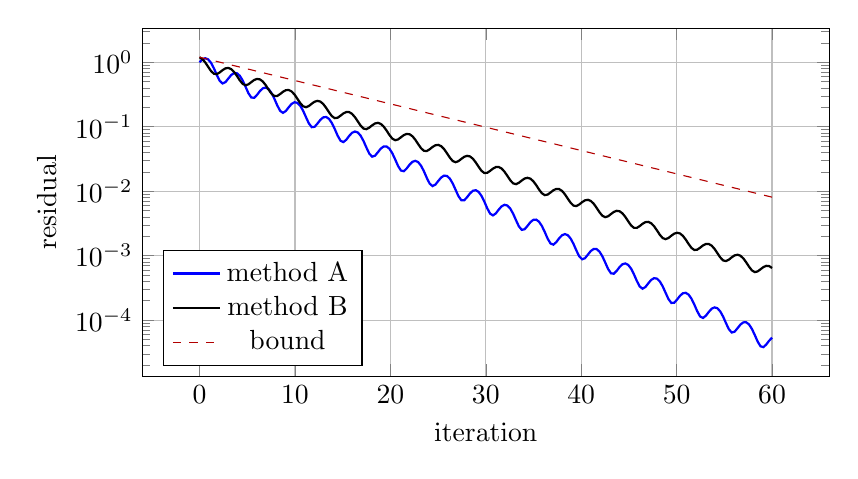
\begin{tikzpicture}\begin{semilogyaxis}[width=0.85\linewidth,height=6cm,xlabel={iteration},ylabel={residual},domain=0:60,grid=major,legend pos=south west]
\addplot[blue,thick,samples=200]{exp(-x/6)*(1+0.3*sin(deg(x*2)))};
\addplot[black,thick,samples=200]{exp(-x/8)*(1+0.2*cos(deg(x*2)))};
\addplot[red!70!black,dashed,samples=200]{1.2*exp(-x/12)};
\legend{method A,method B,bound}
\end{semilogyaxis}\end{tikzpicture}
\caption{Generated figure for \texttt{c9s2-f1} (parameters $a=2$, $b=6$).}\label{fig:c9s2-f1}
\end{figure}

\kant[8-10]

\subsection{Implementation notes}\label{sec:c9s2-i}
The core routine is shown in \cref{lst:c9s2}; its complexity is $\mathcal{O}(N\log N)$ per iteration~\cite{main-31}.

\begin{lstlisting}[language=python,caption={Reference implementation for c9s2.},label={lst:c9s2}]
import numpy as np

def step(u, dt, dx, D):
    """Explicit finite-difference update."""
    lap = (np.roll(u, 1) - 2 * u + np.roll(u, -1)) / dx**2
    return u + dt * D * lap

u = np.exp(-((np.linspace(0, 1, 200) - 0.5) ** 2) / 0.01)
for _ in range(1000):
    u = step(u, 1e-5, 1 / 200, 1.0)
\end{lstlisting}

\kant[3-10]
\begin{theorem}\label{thm:c9s2}
Let $A\in\mathbb{R}^{n\times n}$ be symmetric positive definite with condition number $\kappa$. Then the iteration converges and
$\lVert e_k\rVert_A \le 2\bigl(\tfrac{\sqrt\kappa-1}{\sqrt\kappa+1}\bigr)^k\lVert e_0\rVert_A$.
\end{theorem}
\begin{enumerate}[label=(\roman*)]
\item the bound in \cref{thm:c9s2} is sharp for some initial errors;
\item the constant $2$ cannot be improved in general;
\item preconditioning reduces the effective $\kappa$.
\end{enumerate}

\lipsum[63-63]
